% Energy reconstruction section should have the following sections:
% Shower Reconstruction (Inlucding resoltuion, validation with pi0)
% track reconstruction (Length based methodology, resolution)
%	- Hadronic energy reconstruction (All tracks in a selected neutrino interaction)
% Neutrino Energy Reconstruction

\section{Energy reconstruction}\label{sec:energyreco}

Paragraph here describing general reco strategy: treat the protons and the electron separately.  

\subsection{Electron energy reconstruction and calibration}\label{sec:showerenergy}
The reconstructed energy $E_{reco}^{e}$ of a shower-like object is measured converting the charge of the associated hits into deposited energy in the TPC. It is calculated by multiplying the reconstructed charge ($e^{-}_{reco}$) from hits associated with the reconstructed shower by the calibration factor measured in \cite{michel}:
\begin{equation}
\frac{E_{reco}^{e} \mathrm{(MeV)}}{e^-} = 1.01\frac{e^-}{e^{-}_{reco}} \times \frac{23.6~\mathrm{eV}}{e^-} \times 10^{-6} \frac{\mathrm{eV}}{\mathrm{MeV}} \times \frac{1}{R},\label{eq:calib}
\end{equation}
where:
\begin{itemize}

\item the correction factor $1.01\frac{e^-}{e^{-}_{reco}}$ is obtained measuring the true number of collected electrons $e^{-}$ on the wires using a sample of stopping muons, fitting the $dE/dx$ vs. residual range to values for argon as tabulated by the PDG \cite{pdg},
\item $\frac{23.6~\mathrm{eV}}{e^-}$ is the work function for ionizing an argon atom \cite{workfunction},
\item $R = 0.62$ is the recombination factor obtained with the Modified Box Model \cite{boxmodel}.
\end{itemize}
Figure \ref{fig:ecalib} shows the calibration slope necessary to convert the reconstructed energy $E_{reco}$ into true electron energy $E_{true}$. It has been obtained using only the hits reconstructed in the collection plane. 
The reconstructed energy is obtained summing the hits energy from each reconstructed shower matched to the true electron. The true electron and the reconstructed showers are required to be fully contained within the fiducial volume. Since the reconstructed energy distributions in each true energy bin is asymmetrical, the data points are obtained fitting a Gaussian around the peak of the distribution.
A linear fit of the data points gives:
\begin{equation}
E_{reco}^{e} = 0.78~E^{e} - 0.02~\mathrm{GeV}.
\end{equation}

\begin{figure}[!htbp]
\centering
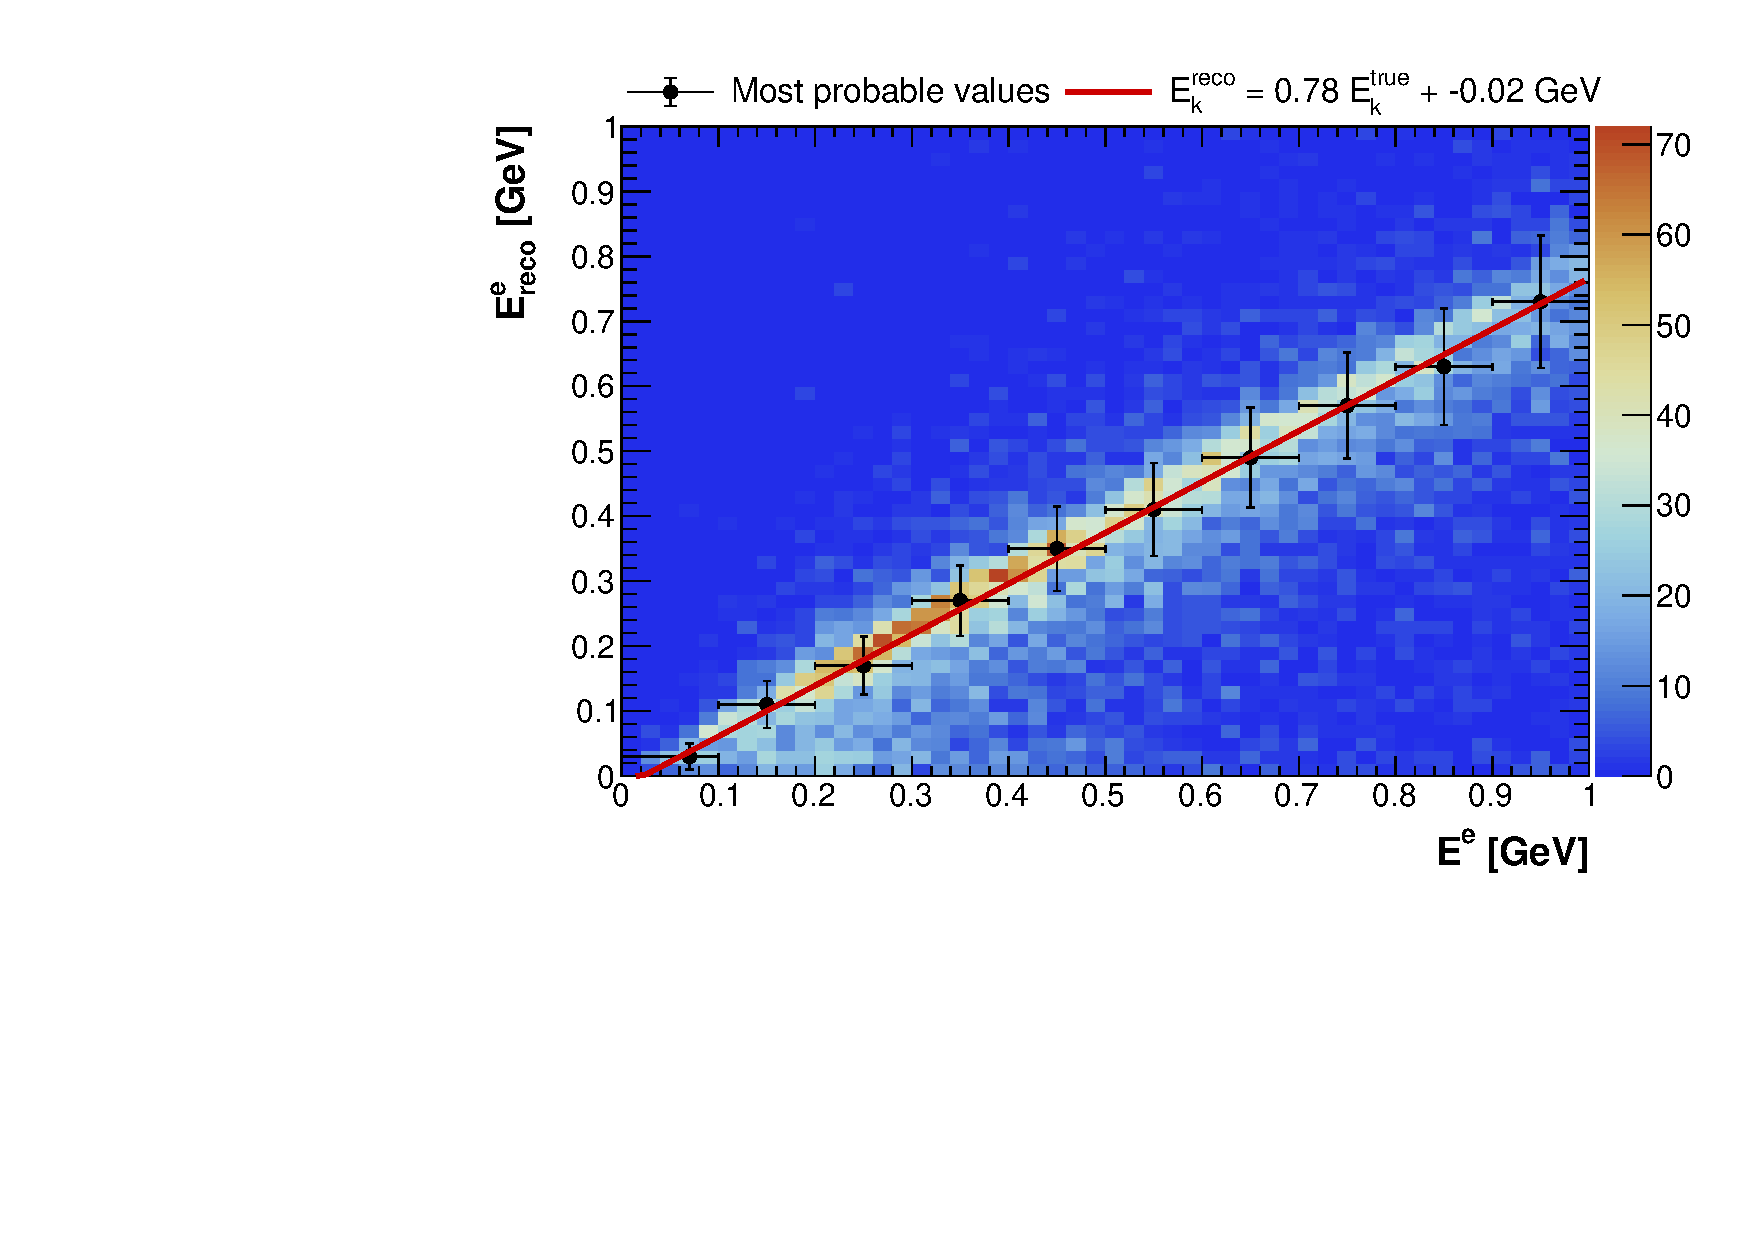
\includegraphics[width=0.65\columnwidth]{figures/ecalib.pdf}
\caption{Bi-dimensional histogram of true electron energy $E^{e}$ vs. reconstructed electron energy $E_{reco}^{e}$. Black points are obtained measuring the most probable value of the $E_{reco}^{e}$ distribution for each $E^{e}$ bin.}
\label{fig:ecalib}
\end{figure}



\subsection{\texorpdfstring{$\pi^0$}{pi0} mass peak}

CC$\pi^0$ events have been studied in order to validate the energy scale and reconstruction in the low-energy region in data as well as in the Monte Carlo. There is no aim for an analysis in the CC$\pi^0$ channel. Instead the purpose is to exploit a pure sample of $\pi^0$ decays, which can be used as standard candle to validate the energy reconstruction.
The samples which have been used are:
\begin{itemize}
  \item Data: hand scanned CC$\pi^0$ sample, which has been already used in \cite{caratelli}
  \item Monte Carlo: BNB + cosmic + generator level requirements:
  	\begin{itemize}
  		\item Selected neutrino matched to a true neutrino
		\item Charged current interaction
		\item Exactly one $\pi^0$ in the final state
  	\end{itemize}
\end{itemize}
The selection relies on the optical selection presented before (ref. to optical selection). Subsequently events are required to have at least two reconstructed showers with hits on the collection plane. The second requirement is meant to remove events with null shower energy, as the energy is computed from the collection plane only. The energy of the showers is calibrated using the energy calibration shown previously (derived from electrons-matched-showers using the Monte Carlo, ref. to this calibration).
The $\pi^0$ candidate is computed starting from the two most energetic showers. The distribution of the number of reconstructed showers in each event is shown in the left plot in fig. \ref{fig:mc_mass_e2} for data and MC.

As there are many events with more than two showers, about two thirds in data and one half in Monte Carlo, a simple re-clustering of the energy is performed. It is meant to recover the energy from broken showers. The two most energetic showers are considered. Then, the energy of any additional shower is summed to the closest in angle among the two most energetic showers. The direction of the two most energetic showers is not modified in this process. The mass is computed from the two most energetic showers, with the energy corrected after the re-clustering, as:
\[ M = \sqrt{E_1 E_2 (1 - \cos\theta)} \]\textbf{}
where $E_1$ and $E_2$ are the energies of the most and the second most energetic showers, respectively. $\theta$ is the 3-D angle between the directions of the two showers.

\begin{figure}[!htbp]
\centering
\begin{minipage}{0.49\columnwidth}
  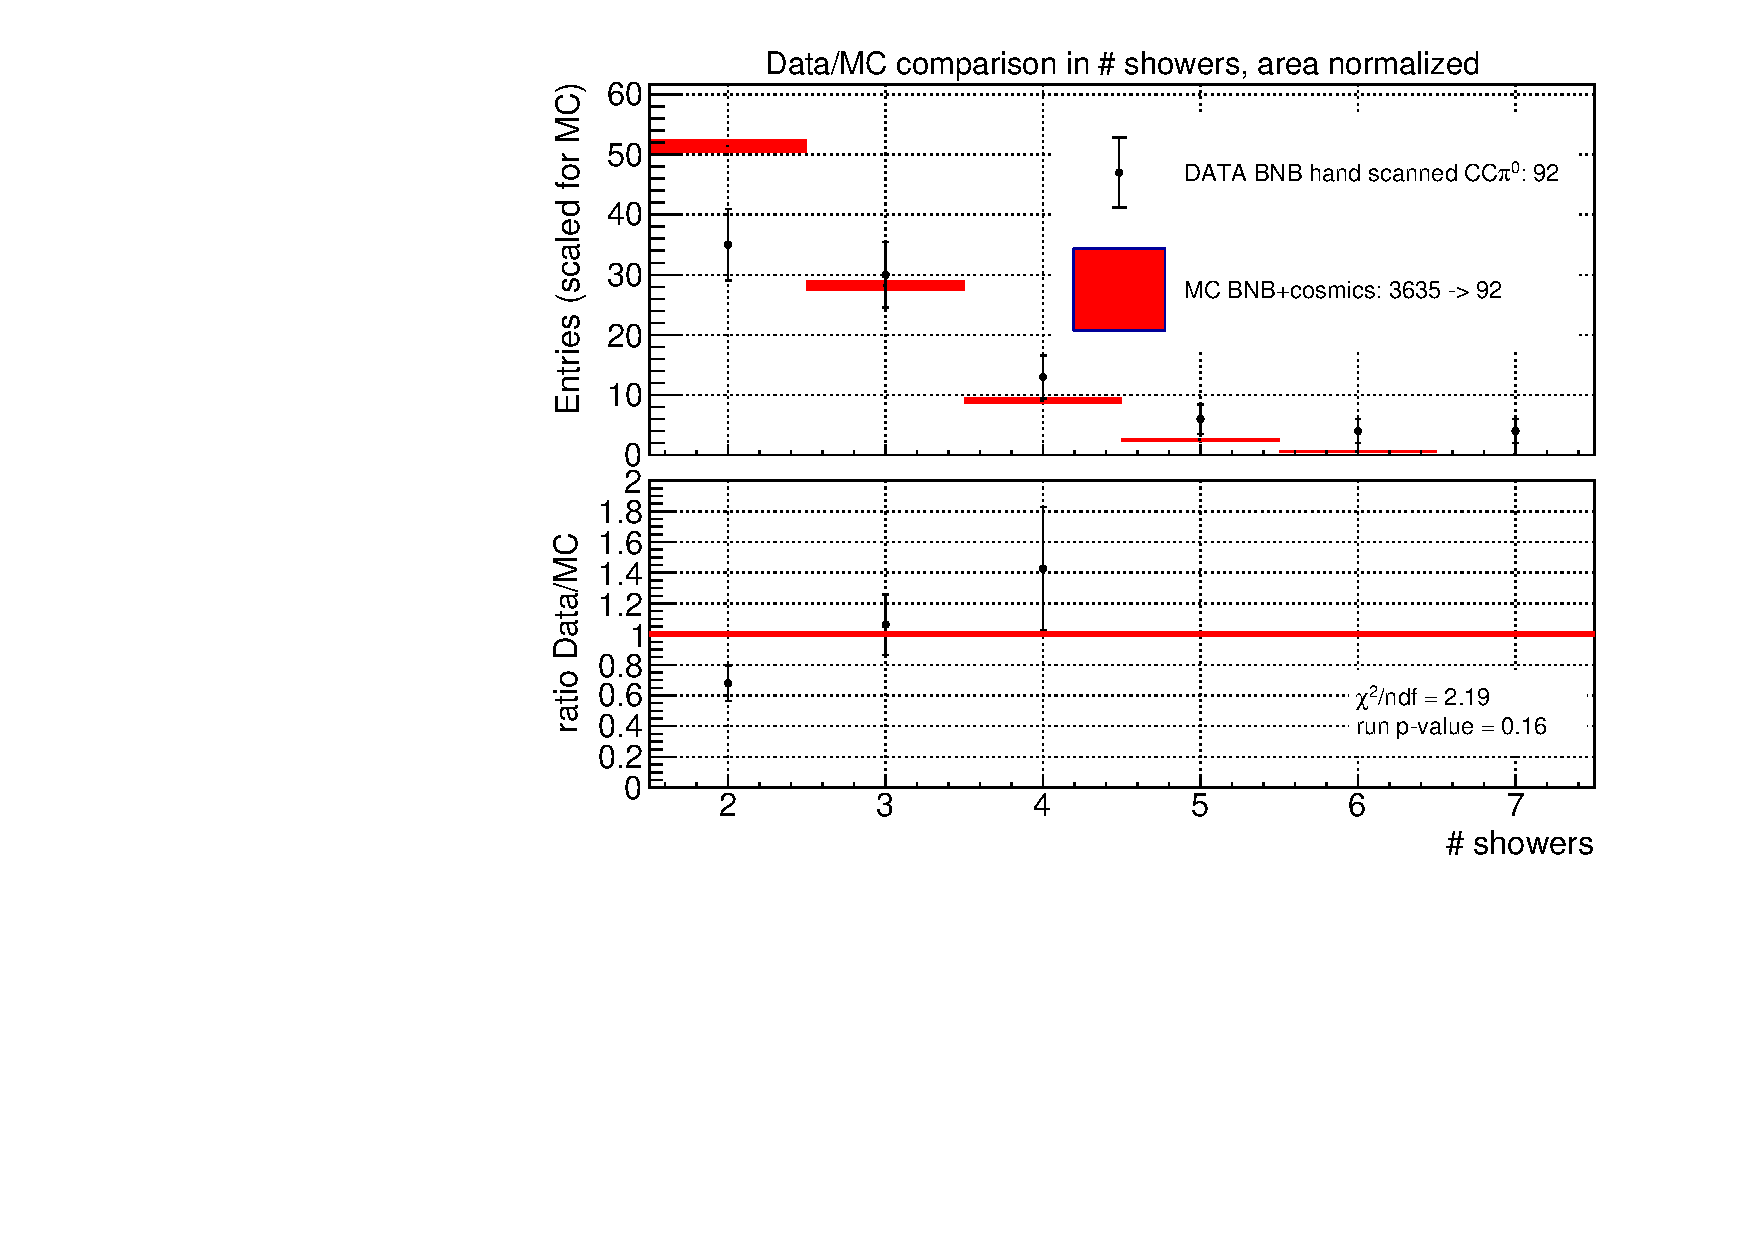
\includegraphics[width=0.99\columnwidth]{_fig/n_showers_data_MC_comparison.pdf}
\end{minipage}
\begin{minipage}{0.49\columnwidth} 
  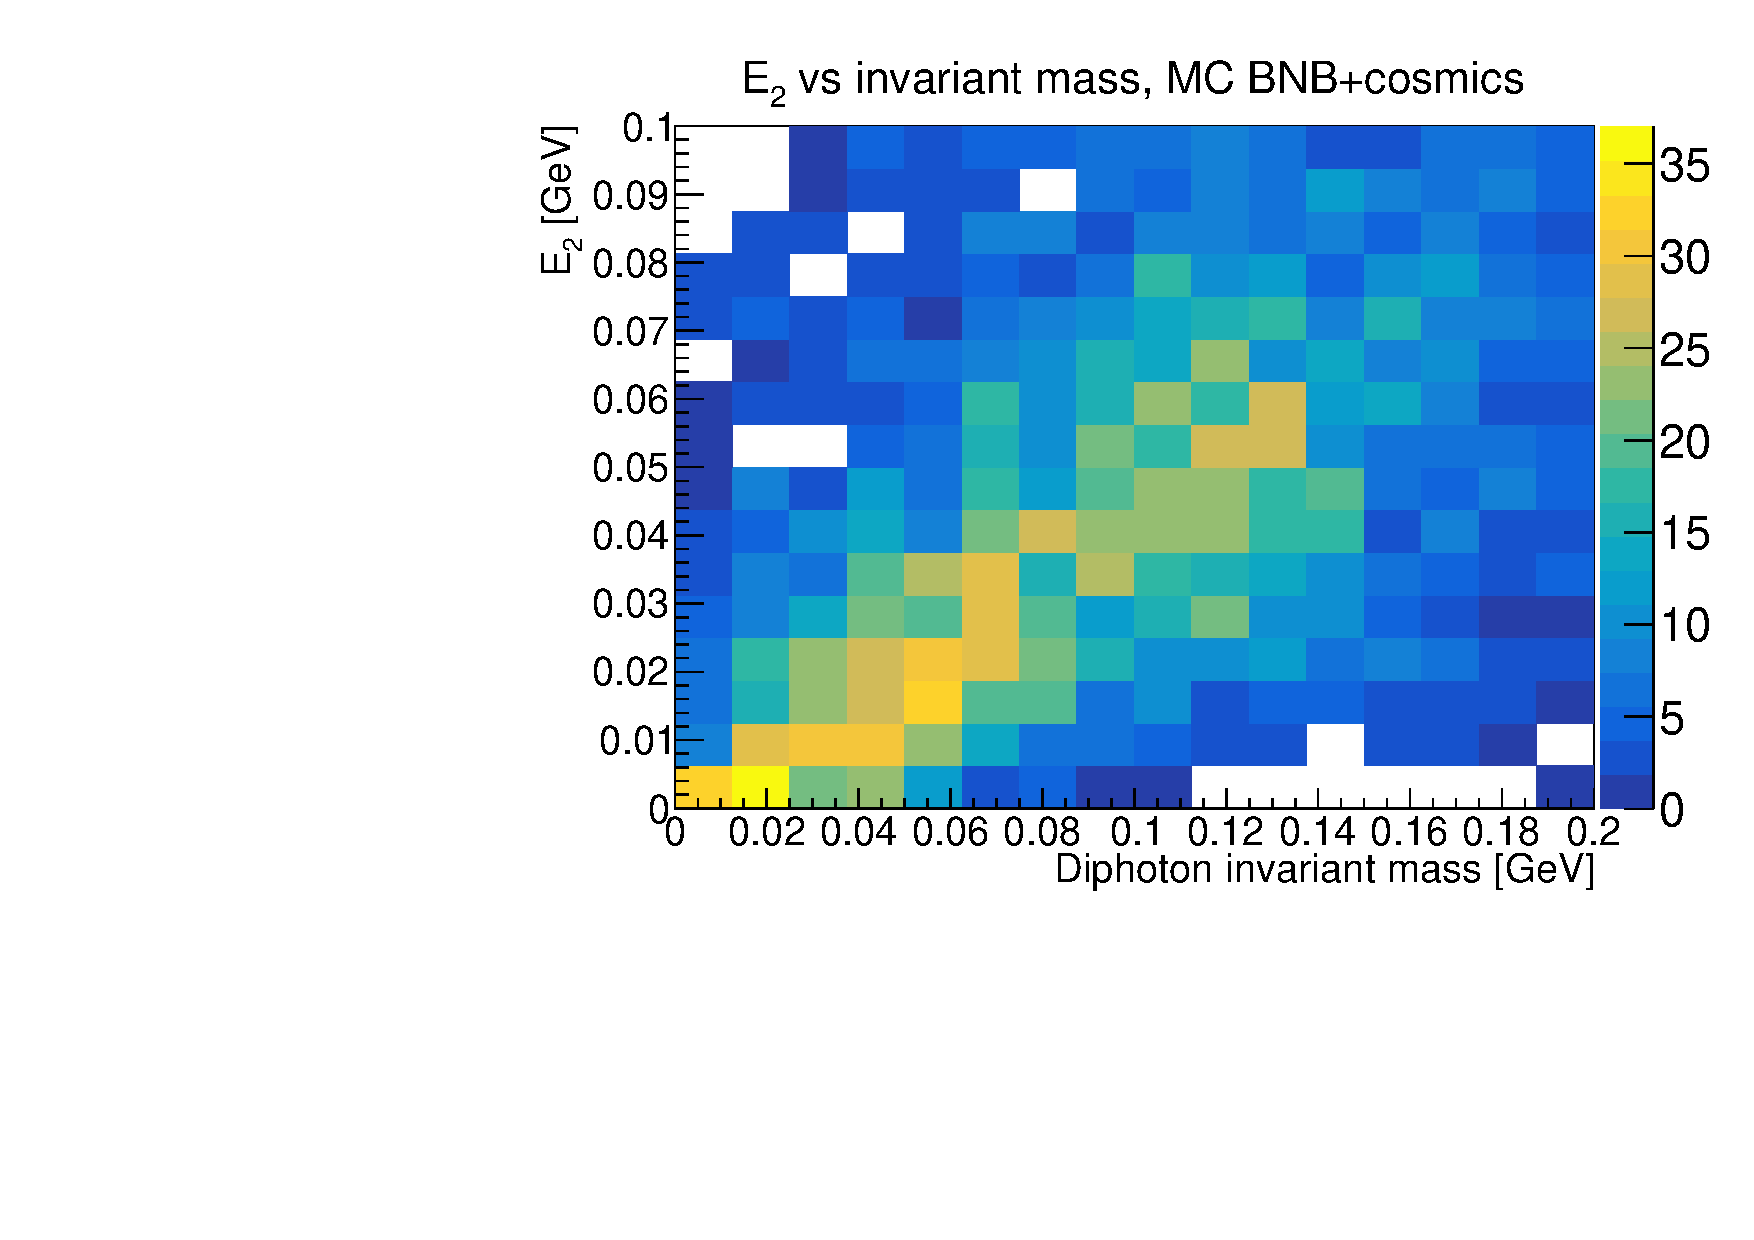
\includegraphics[width=0.99\columnwidth]{_fig/MC_mass_E2.pdf}
\end{minipage}
\caption{Left: Distribution of the number of showers for each event, for data (black dots) and Monte Carlo (red boxes). Right: Bi-dimensional distribution of $E_2$ (y-axis) versus the invariant mass (x-axis) in Monte Carlo events.}
\label{fig:mc_mass_e2}
\end{figure}

In some cases a significant amount of energy is missing. For instance one of the two true showers is missed, and a smaller showers, resulting from noise or from mis-reconstruction of other objects, is taken as one of the decay products of the $\pi^0$. The right plot in figure \ref{fig:mc_mass_e2} shows the bi-dimensional distribution of the invariant mass (x-axis) versus $E_2$ (x-axis) for Monte Carlo events. As it is possible to see, a significant amount of events has small $E_2$ and small mass. Thus, to take into account this effect and remove events with one shower badly or mis-reconstructed, the second most energetic shower is required to have reconstructed energy larger than 30 MeV.

The final peak after the selection is shown in figure \ref{fig:pi0_mass_peak}. The two histograms, for data and Monte Carlo, are fitted through a binned ML fit with a crystal ball function (Gaussian core, $C^1$-matched with a power-law right tail). The fit result, for what concerns the core is:
\[ \text{Data:} \quad \mu = 133 \pm 7~\text{MeV}, \quad \sigma = 47 \pm 5~\text{MeV} \]
\[ \text{Monte Carlo:} \quad \mu = 119 \pm 2~\text{MeV}, \quad \sigma = 51 \pm 2~\text{MeV} \]

The two results are significantly close to the nominal mass of 135~MeV, and shows a relatively good agreement between data and Monte Carlo. However, the discrepancy is significant and requires more investigation, in order to be understood completely.

\begin{figure}[!htbp]
\centering
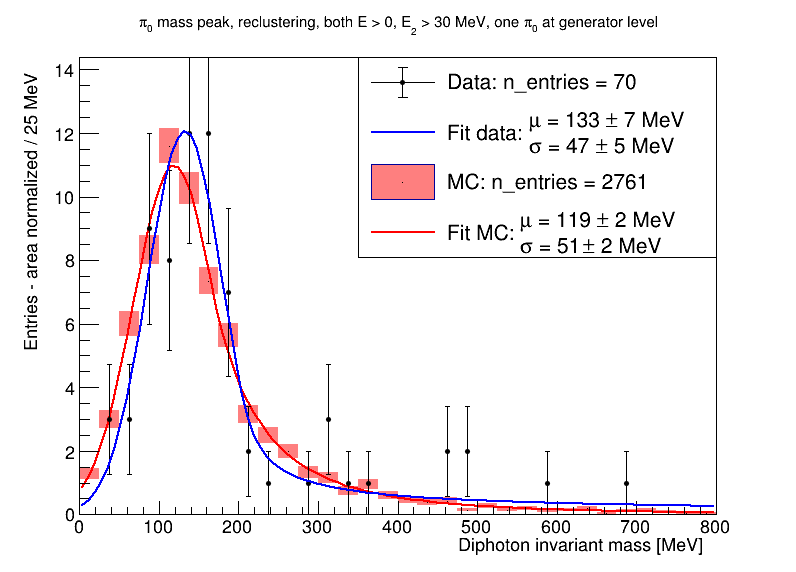
\includegraphics[width=0.8\textwidth]{_fig/data_mc_pi0_mass_peak_crb_cut_on_second_shower.png}
\caption{Diphoton invariant mass distribution for data and Monte Carlo. The two lines show the crystal ball functions as obtained from the ML fit to the two histrograms.} 
\label{fig:pi0_mass_peak}
\end{figure}

\subsection{Hadronic Energy Reconstruction}
\subsubsection{Single Proton energy reconstruction and calibration}

\subsubsection{Neutrino Produced Hadronic Energy Reconstruction}

\subsection{Neutrino Energy Reconstruction}